\chapter{Arhitektura i dizajn sustava}
		
		Arhitektura sustava može se podijelit na tri glavna podsustava: web preglednik, web poslužitelj i baza podataka.
	\begin{itemize}
		\item 	\textbf{Web preglednik} – program koji služi za pristupanje web stranicama. Putem web preglednika korisnik komunicira sa poslužiteljem koristeći princip zahtjev-odgovor ili šalje podatke (najčešće u obliku obrazaca). Daljnja zadaća web preglednika je osigurati da se traženi podaci ispravno prikazuju ili da se ispravno prosljeđuju i spremaju na poslužitelj.
		\item 	\textbf{Web poslužitelj} – glavni je dio web aplikacije. To je most koji povezuje korisnika i bazu podataka koji se temelji na protokolu HTTP. Na zahtjeve korisnika dohvaća tražene podatke (resurse) ili obrađuje i sprema poslane podatke od korisnika.
		\item 	\textbf{Baza podataka} – srce je sustava. U njoj su pospremljeni svi podaci. Skoro ne postoji sustav u kojem nema komunikacije između aplikacije i baze.	
	\end{itemize}
		Aplikacije je izgrađena na modelu MVC (Model – View - Controller) softverske arhitekture. Shodno tome aplikaciju onda dijelimo na tri komponente:
	\begin{itemize}
		\item	\textbf{Model} – glavna komponenta sustava. Čuva razrede čiji se objekti obrađuju.
		\item	\textbf{View} – komponenta zaslužna za reprezentaciju podataka.
		\item	\textbf{Controller} – komponenta zaslužna za komunikaciju između korisnika i modela ili view-a.
	\end{itemize}
	
		\smallskip
		Programski jezik koji smo odabrali za izradu backend-a naše aplikacije je ????, zajedno sa REST API-em za komunikaciju sa bazom. Za izradu fronend-a korišteni su ??????. Od vanjskih servisa smo integrirali podršku za korištenje Google Maps-a. Razvojno okruženje koje smo koristili je bilo Visual Studio Code.
		

		

				
		\section{Baza podataka}
			
			%\textbf{\textit{dio 1. revizije}}\\
			
		%\textit{Potrebno je opisati koju vrstu i implementaciju baze podataka ste odabrali, glavne komponente od kojih se sastoji i slično.}
			U ovom projektu koristit ćemo relacijsku bazu podataka, čije su osnovne jedinke entiteti, definirani imenom i skupom atributa. Osnovna zadaća baze podataka je pohrana podataka te brza i efikasna obrada tih podataka u ovisnosti i korisničkim zahtjevima. U bazi podataka su pohranjeni podaci o korisnicima, njihovim ulogama, preferencijama, kao i o smještaju te dostupnosti smještaja. Dodatno uz navedeno, zbog zahtjeva organizacije prijevoza, baza također sprema informacije o vrstama vozila i dostupnosti tih vozila kao i o vremenu i mjestu boravka korisnika zdravstvenog turizma. Tako su i definirani sljedeći entiteti:
			\begin{itemize}
				\item Clinic
				\item Town
				\item User
				\item Credentials
				\item Role
				\item Patient
				\item Accomodation
				\item AccomodationType
				\item Equipped
				\item AccomodationAvaliability
				\item Transporter
				\item Vehicle
				\item VehicleOccupied
				\item VehicleAvaliability
			\end{itemize}
		
			\subsection{Opis tablica}
			
				%clinic
				\textbf{Clinic} Ovaj entitet sadrži podatke o klinikama u odabranoj zemlji. Atributi su: ClinicID (primary key), clinicName, clinicAddress, TownID (foreign key), latitude i longitude. Ovaj je entitet u vezi Many-to-One sa entitetom Town preko atributa TownID, u Many-to-Many vazi sa entitetom Accomodation preko atributa ClinicID i AccomodationID te u Many-to-Many vezi sa entitetom Transporter preko atributa ClinicID i TransporterID.
				
				\begin{longtblr}[
					label=none,
					entry=none
					]{
						width = \textwidth,
						colspec={|X[6,l]|X[6, l]|X[20, l]|}, 
						rowhead = 1,
					} %definicija širine tablice, širine stupaca, poravnanje i broja redaka naslova tablice
					\hline \SetCell[c=3]{c}{\textbf{Clinic}}	 \\ \hline[3pt]
					ClinicID & INT	& Jedinstveni brojčani identifikator klinike,automatski generiran \\ \hline
					clinicName & VARCHAR & Ime klinike	\\ \hline 
					clinicAddress & VARCHAR & Adresa klinike  \\ \hline 
					Latitude & DECIMAL	& Geografska širina	\\ \hline 
					Longitude & DECIMAL & Geografska visina \\ \hline
				\end{longtblr}
				
				%Town
				\textbf{Town} Ovaj entitet sadrži podatke o gradovima u kojima se nalaze klinike i dolaze pacijenti na liječenje. Atributi su: TownID (primary key) i townName. Ovaj entitet je u vezi One-to-Many sa entitetom Clinic preko atributa TownID i u vezi One-to-Many sa entitetom Accomodation preko atributa TownID i u Many-to-Many vezi sa entitetom Transporter preko atributa TownID.
				
				\begin{longtblr}[
					label=none,
					entry=none
					]{
						width = \textwidth,
						colspec={|X[6,l]|X[6, l]|X[20, l]|}, 
						rowhead = 1,
					} %definicija širine tablice, širine stupaca, poravnanje i broja redaka naslova tablice
					\hline \SetCell[c=3]{c}{\textbf{Town}}	 \\ \hline[3pt]
					TownID & INT & Jedinstveni brojčani identifikator grada, automatski generiran \\ \hline
					townName & VARCHAR & Ime grada	\\ \hline 
				\end{longtblr}
				
				%User
				\textbf{User} Ovaj entitet sadrži podatke o korisnicima aplikacije; svi administratori i oni koji mogu dodavati ili ažurirati ili brisati podatke iz baze. Atributi su: UserID (primary key), PIN(personal identification number), name, surname, contact, email. Ovaj je entitet u vezi Many-to-Many sa entitetom Role preko atributa RoleID.
				
				\begin{longtblr}[
					label=none,
					entry=none
					]{
						width = \textwidth,
						colspec={|X[6,l]|X[6, l]|X[20, l]|}, 
						rowhead = 1,
					} %definicija širine tablice, širine stupaca, poravnanje i broja redaka naslova tablice
					\hline \SetCell[c=3]{c}{\textbf{User}}	 \\ \hline[3pt]
					UserID & INT & Jedinstveni brojčani identifikator korisnika, automatski generiran \\ \hline
					PIN & INT & Identifikacijski broj korisnika	\\ \hline 
					name & VARCHAR & Ime korisnika  \\ \hline 
					surname & VARCHAR & Prezime korisnika	\\ \hline 
					phone & VARCHAR & Broj mobitela korisnika \\ \hline
					email & VARCHAR & Elektronička pošta korisnika \\ \hline
				\end{longtblr}
				
				%Credentials
				\textbf{Credentials} Ovaj entitet sadrži podatke o korisničkim računima administratora. Atributi su: username i password. Ovaj je entitet u One-to-One vezi sa entitetom User preko atributa UserID.
				
				\begin{longtblr}[
					label=none,
					entry=none
					]{
						width = \textwidth,
						colspec={|X[6,l]|X[6, l]|X[20, l]|}, 
						rowhead = 1,
					} %definicija širine tablice, širine stupaca, poravnanje i broja redaka naslova tablice
					\hline \SetCell[c=3]{c}{\textbf{Credentials}}	 \\ \hline[3pt]
					username & VARCHAR & Jedinstveno korisničko ime \\ \hline
					password & BINARY & Lozinka korisnika za prijavu u aplikaciju	\\ \hline 
				\end{longtblr}
				
				%Patient
				\textbf{Patient} Ovaj entitet sadrži podatke o korisnicima zdravstvenog turizma. Atributi su: PatientID (primary key), PIN (personal identification number), name, surname, email, phone, residenceAddress. Ovaj je entitet u vezi Many-to-One sa entitetom Accomodation preko atributa AccomodationID.
				
				\begin{longtblr}[
					label=none,
					entry=none
					]{
						width = \textwidth,
						colspec={|X[6,l]|X[6, l]|X[20, l]|}, 
						rowhead = 1,
					} %definicija širine tablice, širine stupaca, poravnanje i broja redaka naslova tablice
					\hline \SetCell[c=3]{c}{\textbf{Patient}}	 \\ \hline[3pt]
					PatientID & INT & Jedinstveni brojčani identifikator pacijenta, automatski generiran \\ \hline
					PIN & INT & Identifikacijski broj pacijenta	\\ \hline 
					name & VARCHAR & Ime pacijenta  \\ \hline 
					surname & VARCHAR & Prezime pacijenta	\\ \hline 
					phone & VARCHAR & Broj mobitela pacijenta \\ \hline
					email & VARCHAR & Elektronička pošta pacijenta \\ \hline
					residenceAddress & VARCHAR & Mjesto prebivališta pacijenta \\ \hline
				\end{longtblr}
				
				%Accomodation
				\textbf{Accomodation} Ovaj entitet sadrži podatke o smještaju, vrsti smještaja, njegovoj opremljenosti te adresi na kojoj se nalazi kao i koordinatama. Atributi su: AccomodationID (primary key), address, latitude, longitude, active. Ovaj je entitet u vezi Many-to-One sa entitetom Town preko atributa TownID, nadalje u vezi Many-to-One sa entitetom AccomodationType preko atributa TypeID, u vezi Many-to-One sa entitetom Equipped preko atributa EquippedID, u vezi Many-to-One sa entitetom AccomodationAvaliability preko atributa AccomodationID te u vezi One-to-Many sa entitetom Patient preko atributa AccomodationID.
				
				\begin{longtblr}[
					label=none,
					entry=none
					]{
						width = \textwidth,
						colspec={|X[6,l]|X[6, l]|X[20, l]|}, 
						rowhead = 1,
					} %definicija širine tablice, širine stupaca, poravnanje i broja redaka naslova tablice
					\hline \SetCell[c=3]{c}{\textbf{Accomodation}}	 \\ \hline[3pt]
					AccomodationID & INT & Jedinstveni brojčani identifikator smještaja, automatski generiran \\ \hline
					address & VARCHAR & Adresa smještaja	\\ \hline 
					latitude & DECIMAL & Geografska širina  \\ \hline 
					longitude & DECIMAL & Geografska visina	\\ \hline 
					active & BIT & Je li smještaj upotrebljiv \\ \hline
				\end{longtblr}
				
				%AccomodationType
				\textbf{AccomodationType} Ovaj entitet sadrži podatke o tipu smještaja (stan u zgradi, stan u kući, iznajmljeno, u vlasništvu klinike) . Atributi su: TypeID (primary key), type. Ovaj je entitet u One-to-Many vezi s entitetom Accomodation preko atributa TypeID.
				
				\begin{longtblr}[
					label=none,
					entry=none
					]{
						width = \textwidth,
						colspec={|X[6,l]|X[6, l]|X[20, l]|}, 
						rowhead = 1,
					} %definicija širine tablice, širine stupaca, poravnanje i broja redaka naslova tablice
					\hline \SetCell[c=3]{c}{\textbf{AccomodationType}}	 \\ \hline[3pt]
					TypeID & INT & Jedinstveni brojčani identifikator vrste smještaja, automatski generiran \\ \hline
					description & TEXT & Opis vrste smještaja (stan u kući, stan u zgradi, soba u hotelu ili motelu)	\\ \hline 
				\end{longtblr}
				
				%Equipped
				\textbf{Equipped} Ovaj entitet sadrži podatke o vrsti opremljenosti smještaja (potpuno opremljen, djelomično opremljen).  Atributi su: EquippedID (primary key), equipment. Ovaj je entitet u One-to-Many vezi sa entitetom Accomodation preko atributa EquippedID.
				
				\begin{longtblr}[
					label=none,
					entry=none
					]{
						width = \textwidth,
						colspec={|X[6,l]|X[6, l]|X[20, l]|}, 
						rowhead = 1,
					} %definicija širine tablice, širine stupaca, poravnanje i broja redaka naslova tablice
					\hline \SetCell[c=3]{c}{\textbf{Equipped}}	 \\ \hline[3pt]
					EquippedID & INT & Jedinstveni brojčani identifikator opremljenosti smještaja, automatski generiran \\ \hline
					equipment & TEXT & Opis opremljenosti smještaja (potpuno opremljen, djelomično opremljen)	\\ \hline 
				\end{longtblr}
				
				%AccomodationAvaliability
				\textbf{AccomodationAvaliability} Ovaj entitet sadrži podatke o dostupnosti smještaja za naseljavanje za vrijeme medicinskog boravka. Atributi su: since, till. Ovaj je entitet u One-to-Many vezi sa entitetom Accomodation preko atributa AccomodationID.
				
				\begin{longtblr}[
					label=none,
					entry=none
					]{
						width = \textwidth,
						colspec={|X[6,l]|X[6, l]|X[20, l]|}, 
						rowhead = 1,
					} %definicija širine tablice, širine stupaca, poravnanje i broja redaka naslova tablice
					\hline \SetCell[c=3]{c}{\textbf{AccomodationAvaliability}}	 \\ \hline[3pt]
					since & DATE & Datum od kojeg je smještaj dostupan \\ \hline
					till & DATE & Datum do kojeg je smještaj dostupan \\ \hline 
				\end{longtblr}
				
				%Transporter
				\textbf{Transporter} Ovaj entitet sadrži podatke o prijevoznicima s kojima klinika ima ugovore za prijevoz pacijenata. Atributi su: TransporterID (primary key), organisationName, contact, address, active. Ovaj je entitet u Many-to-Many vezi sa entitetom Town preko atributa TownID, u Many-to-Many vezi sa entitetom Clinic preko atributa ClincID te u One-to-Many vezi sa entitetom Vehicle preko atributa TransporterID.
				
				\begin{longtblr}[
					label=none,
					entry=none
					]{
						width = \textwidth,
						colspec={|X[6,l]|X[6, l]|X[20, l]|}, 
						rowhead = 1,
					} %definicija širine tablice, širine stupaca, poravnanje i broja redaka naslova tablice
					\hline \SetCell[c=3]{c}{\textbf{Transporter}}	 \\ \hline[3pt]
					TransporterID & INT & Jedinstveni brojčani identifikator prijevoznika, automatski generiran \\ \hline
					organisationName & VARCHAR & Ime prijevoznika \\ \hline
					phone & VARCHAR & Broj mobitela prijevoznika \\ \hline
					address & VARCHAR & Adresa baze prijevoznika \\ \hline
					active & BIT & Je li prijevoznik radi \\ \hline
				\end{longtblr}
				
				%Vehicle
				\textbf{Vehicle} Ovaj entitet sadrži podatke o vozilima kojima transporter raspolaže. Atributi su: VehicleID (primary key), typeOf, capacity te active. Ovaj je entitet u Many-to-One vezi sa entitetom Transporter preko atributa TransporterID, u Many-to-Many vezi sa netitetom VehicleOccupied preko atributa VehicleID te u Many-to-Many vezi sa entitetom VehicleAvaliability preko atributa VehicleID.
				
				\begin{longtblr}[
					label=none,
					entry=none
					]{
						width = \textwidth,
						colspec={|X[6,l]|X[6, l]|X[20, l]|}, 
						rowhead = 1,
					} %definicija širine tablice, širine stupaca, poravnanje i broja redaka naslova tablice
					\hline \SetCell[c=3]{c}{\textbf{Vehicle}}	 \\ \hline[3pt]
					VehicleID & INT & Jedinstveni brojčani identifikator vozila, automatski generiran \\ \hline
					typeOf & VARCHAR & Vrsta vozila (kombi, auto) \\ \hline
					capacity & SMALLINT & Kapacitet vozila (2 osobe, 4 osobe, 5 osoba….) \\ \hline
					active & BIT & Je li vozilo u funkciji \\ \hline
				\end{longtblr}
				
				%VehicleOccupied
				\textbf{VehicleOccupied} Ovaj entitet sadrži podatke o vremenima kada je koje vozilo zauzeto, tj. kada prevozi pacijente od smještaja do klinike te natrag to smještaja. Atributi su: timeStart, timeEnd, PatientID. Ovaj je entitet u Many-to-Many vezi sa entitetom Vehicle preko atributa VehicleID te u One-to-One vezi sa entitetom Patient preko atributa PatientID.
				
				\begin{longtblr}[
					label=none,
					entry=none
					]{
						width = \textwidth,
						colspec={|X[6,l]|X[6, l]|X[20, l]|}, 
						rowhead = 1,
					} %definicija širine tablice, širine stupaca, poravnanje i broja redaka naslova tablice
					\hline \SetCell[c=3]{c}{\textbf{VehicleOccupied}}	 \\ \hline[3pt]
					timeStart & TIME & Vrijem od kada je vozilo zauzeto \\ \hline
					timeEnd & TIME & Vrijeme do kada je vozilo zauzeto \\ \hline
				\end{longtblr}
				
				%VehicleAvaliability
				\textbf{VehicleAvaliability} Ovaj entitet sadrži podatke o vremenima kada je koje vozilo dostupno, tj. radno vrijeme radnih dana. Atributi su: DOW (day of the week), tiemStart, timeEnd. Ovaj je entitet u Many-to-Many vezi sa entitetom Vehicle preko atributa VehicleID.
				
				\begin{longtblr}[
					label=none,
					entry=none
					]{
						width = \textwidth,
						colspec={|X[6,l]|X[6, l]|X[20, l]|}, 
						rowhead = 1,
					} %definicija širine tablice, širine stupaca, poravnanje i broja redaka naslova tablice
					\hline \SetCell[c=3]{c}{\textbf{VehicleAvaliability}}	 \\ \hline[3pt]
					DOW & SMALLINT & Dan u tjednu u kojem je vozilo slobodno \\ \hline
					timeStart & TIME & Vrijem od kada je vozilo slobodno \\ \hline
					timeEnd & TIME & Vrijeme do kada je vozilo slobodno \\ \hline
				\end{longtblr}
				
			\subsection{Dijagram baze podataka}
				\begin{figure}[H]
					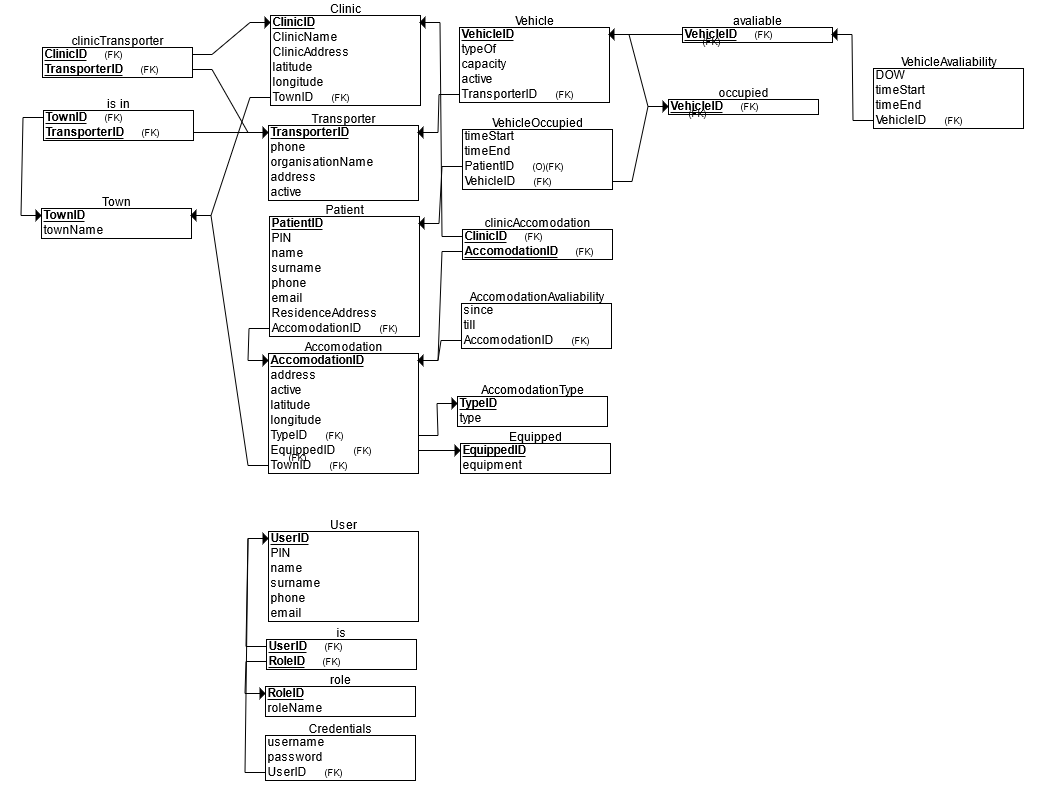
\includegraphics[width=\textwidth]{slike/DB_scheme.PNG} %veličina u odnosu na širinu linije
					\caption{Slika sheme baze podataka}
					\label{fig:db_scheme} %label mora biti drugaciji za svaku sliku
				\end{figure}
			
			\eject
			
			
		\section{Dijagram razreda}
		
			\textit{Potrebno je priložiti dijagram razreda s pripadajućim opisom. Zbog preglednosti je moguće dijagram razlomiti na više njih, ali moraju biti grupirani prema sličnim razinama apstrakcije i srodnim funkcionalnostima.}\\
			
			\textbf{\textit{dio 1. revizije}}\\
			
			\textit{Prilikom prve predaje projekta, potrebno je priložiti potpuno razrađen dijagram razreda vezan uz \textbf{generičku funkcionalnost} sustava. Ostale funkcionalnosti trebaju biti idejno razrađene u dijagramu sa sljedećim komponentama: nazivi razreda, nazivi metoda i vrste pristupa metodama (npr. javni, zaštićeni), nazivi atributa razreda, veze i odnosi između razreda.}\\
			
			\textbf{\textit{dio 2. revizije}}\\			
			
			\textit{Prilikom druge predaje projekta dijagram razreda i opisi moraju odgovarati stvarnom stanju implementacije}
			
			
			
			\eject
		
		\section{Dijagram stanja}
			
			
			\textbf{\textit{dio 2. revizije}}\\
			
			\textit{Potrebno je priložiti dijagram stanja i opisati ga. Dovoljan je jedan dijagram stanja koji prikazuje \textbf{značajan dio funkcionalnosti} sustava. Na primjer, stanja korisničkog sučelja i tijek korištenja neke ključne funkcionalnosti jesu značajan dio sustava, a registracija i prijava nisu. }
			
			
			\eject 
		
		\section{Dijagram aktivnosti}
			
			\textbf{\textit{dio 2. revizije}}\\
			
			 \textit{Potrebno je priložiti dijagram aktivnosti s pripadajućim opisom. Dijagram aktivnosti treba prikazivati značajan dio sustava.}
			
			\eject
		\section{Dijagram komponenti}
		
			\textbf{\textit{dio 2. revizije}}\\
		
			 \textit{Potrebno je priložiti dijagram komponenti s pripadajućim opisom. Dijagram komponenti treba prikazivati strukturu cijele aplikacije.}